\title{Project Proposal}
\author{
	Oliver Little \\
	2011802
}
\date{\today}

\documentclass[12pt]{article}

\usepackage{graphicx}

\graphicspath{{./images}}

% This line sets the text as sans-serif
\renewcommand{\familydefault}{\sfdefault}

\begin{document}
	\maketitle
	
	\section{General Topic}
	
	My project topic falls within the field of distributed systems. I would like to find ways of increasing data processing speed for large datasets (at least 100GB). This sort of processing is generally best applied to ETL \textit{(extract-transform-load)} workflows, where some large dataset needs to be imported, processed in some way, then loaded elsewhere for further analysis. \medskip
	
	Single systems begin to struggle with this volume of data, as it cannot all be loaded into memory at once. Furthermore, often the processing to be performed acts on a small number of rows of data at a time. This means that while the overall dataset is extremely large, the work to be performed lends itself quite well to parallelisation, as only a small number of rows are necessary at any one time.
	
	\section{Problem Definition}
	
	My aim is to build a framework on which data processing operations can be performed on a distributed cluster of nodes. These operations will include typical SQL commands, including:
	\begin{itemize}
		\item Filters
		\item Joins
		\item Group Bys
	\end{itemize}

	As part of the role I performed on my placement year, I had to spend a significant time actually executing the models we had written, as the data regularly changed format, slowing down the data ingestion process. Therefore, I would also like to build some tools into the framework to automate the following workflow:
	\begin{itemize}
		\item Ingesting new data
		\item Performing data processing
		\item Providing alerts for any execution issues
		\item Outputting the results
	\end{itemize}
	Based on the above description, the planned system will feature a number of core components. A UML diagram is included below showing how these will link together, followed by further information on each component:
	
	\begin{center}
		\makebox[\textwidth]{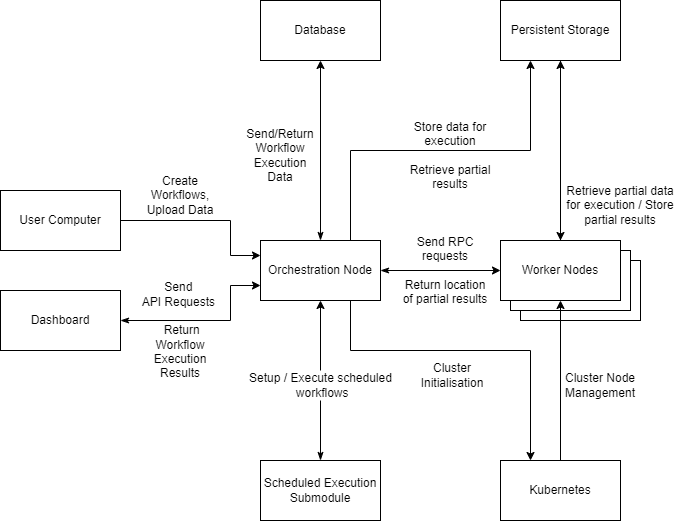
\includegraphics[width=\textwidth]{HighLevelDiagram}}
	\end{center}
	
	\paragraph{Orchestration Node}
	An orchestration node will be the main access point for the system, and will provide functionality over a REST API. It will take all data processing instructions (workflows), and the location of all files to execute on. This node will perform all activities related to starting, managing, and collating the results of the calculation. \medskip
	
	More specifically, it will send instructions to each worker node (using RPC) on what processing to perform on which parts of the full dataset, it will handle restarting any failed nodes and ensuring calculations are fully complete in this case, and it will combine the partial results from all worker nodes to produce the final output. The orchestration node will also need access to an on-disk database in order to store and update the results of workflow executions.
	
	Furthermore, the orchestration node will feature a submodule that will allow it to perform scheduled and repeated executions of workflows, and potentially watch a given file location for changes to initiate a workflow automatically.
	
	\paragraph{Worker Nodes}
	The system will feature a number of worker nodes. Each node will be provided the instructions to execute, and a subset of the entire dataset. It will execute the instructions on the data, persist the results to disk, then send the location of the results to the orchestration node. Dynamic load balancing can be implemented here, as each node will be provided only a small subset of data to execute, then request more work as required.
	
	The worker nodes will be managed using a Kubernetes or Docker Swarm cluster.
	
	\paragraph{File Storage}
	The system will feature a distributed file storage component. This will aim to provide resiliency against hard drive failure, while also improving file access times by storing data in locations close to the worker nodes. I haven't yet decided whether this will use an existing solution like HDFS, or if I will implement my own. My main goal with this component is to provide quick access times to data that can be grouped by a unique key, which means some kind of index might be the only thing that is necessary.
	
	\paragraph{Dashboard}
	The dashboard will provide a convenient frontend for the user to access workflows they have created, including information on previous executions, and will allow the user to initiate instant and scheduled executions.
	
	\section{Previous Work}

	This area is well researched, and many solutions already exist with varying advantages and disadvantages:
	
	\paragraph{MapReduce}
	Google’s MapReduce is an framework designed to perform parallelised data processing using two operations - map, and reduce. It is an extremely simple framework to use, but from the research I have performed so far, contains two key weaknesses. Firstly, it performs many save and load operations to disk. This provides significant resiliency to both node and disk failure (as it utilises HDFS for resilient file storage), but it also significantly slows down processing compared to retaining data in-memory. Furthermore, the API does not transfer well to data that needs to be processed as a group according to some key.
	
	\paragraph{Apache Spark}
	Apache Spark is another alternative which solves problems much closer to what I'm trying to achieve. It provides higher-level API, including both Panda DataFrames, and SQL APIs. However, it again struggles with grouped data, and also has some issues with large datasets as it attempts to store as much of the data as possible in memory
	
	\section{Potential Challenges and Difficulties}
	
	I foresee a number of interesting challenges I will need to solve as part of this project:
	
	\begin{enumerate}
		\item Setting up and managing the cluster
		\begin{itemize}
			\item I expect to use an existing framework for initialising and managing both the main and worker nodes, like Kubernetes or Docker Swarm.
			\item However, while this means I will not have to consider challenges like restarting failed nodes from a container perspective, there will still be other resilience considerations like ensuring the task completes successfully when a node fails. % make this clearer (i.e.: recalculating data for failed nodes)
		\end{itemize}
		\item Storage of Data % need to change this to mention that this needs to be investigated further
		\begin{itemize}
			\item I haven't yet decided whether I will be using an existing distributed file storage solution like HDFS or developing my own, as there are a number of interesting problems to solve here, and it could result in significant performance benefits for the framework.
			\item However, including this as a task to complete will be a significant amount of work on its own.
		\end{itemize}
		\item Loan balancing and optimisation
		\begin{itemize}
			\item Loan balancing will need to be implemented to ensure that work is allocated to effectively use all nodes' resources.
			\item There will need to be a significant amount of optimisation performed across the project, including getting the data from disk, performing the actual processing, and compiling the results.
		\end{itemize}
		\item Test data
		\begin{itemize}
			\item I will not be able to use any data from my placement role due to confidentiality issues.
			\item However, it should be relatively straightforward to generate test data for the existing use cases, as they are very well defined and I have prior experience working with the data. These use cases include recalculating interest on loans, and recalculating transaction fees.
		\end{itemize}
	\end{enumerate}
	
	\section{Methodology}
	I plan to implement the tool in Scala. This is because it features the structured object-orientation that Java also provides, but includes some features from functional languages which might prove useful. 
	
	I will also use either Kubernetes or Docker Swarm to handle the cluster management, and I have yet to decide whether I will be using an existing distributed file system for retaining the data on disk.
	
	I will be following an Agile methodology when creating my project, splitting development into sprints. These will likely be broken down by week
	
	\section{Major Milestones}
	Some key milestones for my project include:
	\begin{itemize}
		\item \textbf{Project Inspection/End of Term 1:} Storage solution for data implemented, early Orchestration + Worker Nodes setup created, user able to make simple requests and collate the results. Written up first draft of 'Motivation \& Aims' section of project report.
		\item \textbf{End of December:} Full Orchestration + Worker Nodes setup implemented, including resilience measures for failed nodes. Written up first draft of 'Methodology' section of project report.
		\item \textbf{End of February:} Dashboard and Scheduled Execution Submodule written
		\item \textbf{Project Demonstrations:} Code bugfixes, performed performance and user testing. Written up first draft of 'Results' section of project report.
		\item \textbf{Project Submission Date:} Written up 'Evaluation' section and final editing of project report.
	\end{itemize}
	
	% 5 bullets on major milestones for the project (both code and documentation)
	%should link in with proposed structure
	% e.g: create cluster instantiation
	% sending data to nodes
	% storage solution
	% collating results from nodes
	% orchestration node
	%maybe some milestones include going back to others
	
	\section{Specialism and Competencies}
	\small{\textit{This section is specific to the degree apprenticeship requirements.}} \medskip
	
	I have selected the Software Engineer specialism to complete as part of my project. While my project contains some networking and data analysis elements, the majority of it is focused around creating a large piece of software, following best software engineering practices.
	Included below is a list of the competencies required as part of the Software Engineer specialism, and how I intend to meet each one:
	
	% can link in with team project, speaking back to pwc, etc
	
	\begin{enumerate}
		\item \textbf{Create effective and secure software solutions using contemporary software development languages to deliver the full range of functional and non-functional requirements using relevant development methodologies:} 
		I will determine the functional and non-functional requirements for my project before beginning implementation. I will use the MoSCoW method \textit{(must-should-could)} in order to prioritise which requirements to meet first. 
		\item \textbf{Undertake analysis and design to create artefacts, such as use cases to produce robust software designs:} 
		I will perform analysis on how my project will be used in order to determine any functional and non-functional requirements that should be met.
		\item \textbf{Produce high quality code with sound syntax in at least one language following best practices and standards:} 
		I will be developing my project using a language with object-oriented features, and will ensure my code follows best practices and standards for that language.
		\item \textbf{Perform code reviews, debugging and refactoring to improve code quality and efficiency:} I will make use of Git while developing my project, which will allow me to easily refactor my code. Furthermore, my repository will be hosted on GitLab, where I can review my own code changes before merging them.
		\item \textbf{Test code to ensure that the functional and non-functional requirements have been met:}
		I will perform both unit and integration testing using automated testing frameworks to ensure my code is thoroughly tested.
		\item \textbf{Deliver software solutions using industry standard build processes, and tools for configuration management, version control and software build, release and deployment into enterprise environments:}
		I will make use of Git for version control, and if possible use CI/CD pipelines for building and deploying test environments of my project. I will also aim to use CI/CD to automatically run my unit tests on each commit.
		\item \textbf{How to operate at all stages of the software development lifecycle:}
		I will follow Agile methodology while developing my project, but will also spend some time before beginning development to investigate existing solutions and create a high-level design of the architecture.
		\item \textbf{How teams work effectively to develop software solutions embracing agile and other development approaches:} \textit{While I will be working on my own during this project, I have had previous experience with this competency during the Team Project module during second year, and I will also maintain contact with the team I worked with during my placement year to gain advice and feedback on the system I am building.}
		\item \textbf{How to apply software analysis and design approaches:} \textit{I have previous experience of this competency from the Software Engineering module in second year, and I will apply the skills I gained to this project to design a maintainable system.}
		\item \textbf{How to interpret and implement a design, compliant with functional, non-functional and security requirements:} \textit{I will be writing functional and non-functional requirements before beginning development, and I will use the requirements I write in order to aid my implementation.}
		\item \textbf{How to perform functional and unit testing:} I will use automated test frameworks to write and execute unit tests.
		\item \textbf{How to use and apply the range of software tools used in Software Engineering:} I will make use of many tools used in Software Engineering, including Git, automated test frameworks and CI/CD pipelines.
	\end{enumerate}
\end{document}

